\section{Alakkal záró kötések}%###############################################################

\subsection{Előfeszítési háromszög}%============================================================

\begin{wrapfigure}{R}{.28\textwidth}
	\centering
	\vspace{-3cm}
	\begin{subfigure}{\linewidth}
		\centering
		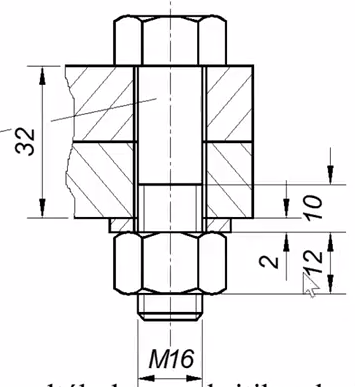
\includegraphics[width=.7\linewidth, trim=0 4 0 0, clip]{elof-hszog}
		\caption{Csavarkötés}
	\end{subfigure}\\[3mm]
	\begin{subfigure}{\linewidth}
		\centering
		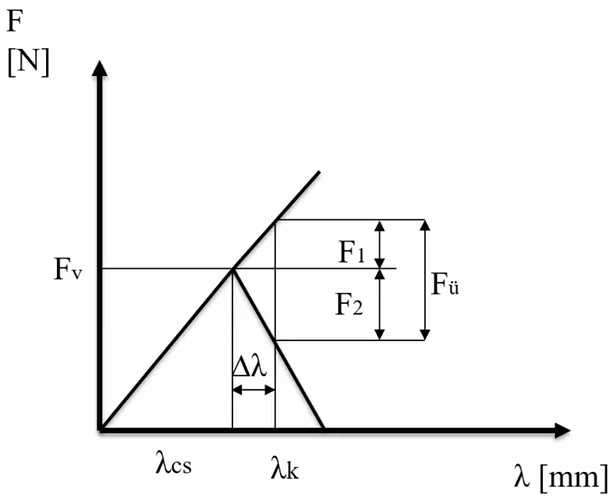
\includegraphics[width=\linewidth]{hszog-hatasabra}
		\caption{Előfeszítési háromszög}
	\end{subfigure}
	\caption{Csavarkötés méretezése}
\end{wrapfigure}
\parbox{.65\textwidth}{
\begin{outline}
	\1 adatok
		\2 $F_\text{max} = 6000$ N
		\2 $\mu = 0.14$
		\2 a közrefogott elemeket egy csőnek tekintjük, $d_\text{cs}=18$ mm, $D_\text{cs}=45$ mm méretekkel
		\2 $d_2 = 14.701$ mm
		\2 a kritikus lazító erő az üzemi erő kétszerese
		\2 Mekkora a beállított előfeszítő erő?
		\2 Mekkora lesz a csavarban ébredő legnagyobb erő?
\end{outline}}
\begin{outline}
	\1 megoldás
		\2 $F_\text{ü} = \frac{2F}{n} = 3000$ N (egy csavarra)
		\2 $F_\text{krit} = 2F_\text{ü} = 6000$ N
		\2 $F_1 = \frac{s_\text{cs}}{s_\text{cs}+s_\text{k}}F_\text{ü}$ 
		\2 $F_2 = \frac{s_\text{k}}{s_\text{cs}+s_\text{k}}F_\text{ü}$ 
		\2 $s_\text{cs}$ és $s_\text{k}$ a csavar és a közrefogott elemek rugómerevsége
		\2 csavar rugómerevsége
			\3 $s_\text{cs} = \frac{F_\text{v}}{\lambda_\text{cs}}=\frac{E}{\sum\frac{l_i}{A_i}}$
			\3 menetes rész
				\4 $A_\text{m} = \frac{d_2^2\pi}{2} = 169.74\text{ mm}^2$
				\4 $l_\text{m} = 14$ mm
			\3 menet nélküli rész
				\4 $A_\text{nm} = \frac{d^2\pi}{2} = 201.06\text{ mm}^2$
				\4 $l_\text{nm} = 24$ mm
			\3 $s_\text{cs} = 1.02\cdot 10^6~\frac{\text{N}}{\text{mm}}$
		\2 közrefogott elemek rugómerevsége
			\3 $s_\text{k} = \frac{A_\text{k}E}{l_\text{k}}$
			\3 $A_\text{k} = 1336\text{ mm}^2$
			\3 $s_\text{k} = 8.77\cdot 10^6~\frac{\text{N}}{\text{mm}}$
		\2 $F_\text{v} = 5375$ N
		\2 $F_1 = 312$ N
		\2 $F_{1\text{max}} = F_\text{v}+F_1 = 5687$ N
\end{outline}

\subsection{Szegecskötés}%============================================================

\begin{wrapfigure}{R}{.28\textwidth}
	\centering
	\vspace{-3cm}
	\centering
	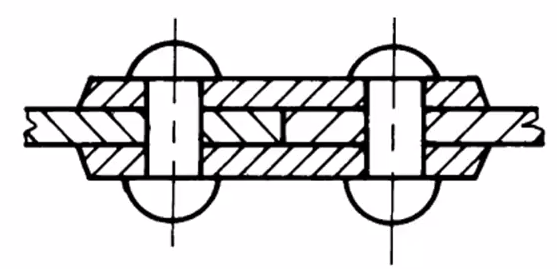
\includegraphics[width=\linewidth]{hevederes-szegecs}
	\caption{Hevederes szegecskötés}
\end{wrapfigure}
\parbox{.7\textwidth}{
\begin{outline}
	\1 adatok
		\2 a lemez vastagsága $v =20$ mm
		\2 $d_\text{szegecs} = 5$ mm
		\2 $\tau_\text{max} = 70$ MPa
		\2 $p_\text{max} = 140$ MPa
		\2 $\sigma_\text{max} = 190$ MPa
		\2 a lemez szélessége $l=60$ mm
		\2 Mekkora a maximális húzóerő?
\end{outline}}
\begin{outline}
	\1 megoldás (átlapolt szegecskötés, járulékos hajlítás nélkül)
		\2 nyíró igénybevétel
			\3 $\tau = \frac{T_\tau}{A_\tau}$
			\3 $A_\tau = \frac{d^2\pi}{4}z = 78.5\text{ mm}^2$
			\3 $F_\tau^\text{max} = \tau_\text{meg}A_\tau = 5495$ N
		\2 felületi nyomás
			\3 $p=\frac{F_\text{p}}{A_\text{p}}$
			\3 $A_\text{p} = dvz = 400\text{ mm}^2$
			\3 $F_\text{p}^\text{max} = p_\text{meg}A_\text{p} = 56000$ N
		\2 különlegességek: szállítófeszültség
			\3 lemez felület: $A_\sigma = v(l-zd)=1800\text{ mm}^2$
			\3 $F_\sigma=\sigma_\text{meg}A_\sigma=152000$ N
		\2 $F_\text{meg} = \min(F_i) = F_\tau=5495$ N
	\1 megoldás (hevederes szegecskötés)
		\2 átlapoló lemezek vastagsága $v_2 = 6$ mm
		\2 nyíró igénybevétel
			\3 $A_\tau = 157\text{ mm}^2$
			\3 $F_\tau^\text{max} = 10990$ N
		\2 felületi nyomás
			\3 $A_{\text{p}1} = dvz = 400\text{ mm}^2$
			\3 $A_{\text{p}2} = 2dv_2z = 240\text{ mm}^2$
			\3 $F_\text{p}^\text{max} = p_\text{meg}A_\text{p}^\text{min} = 31600$ N
		\2 különlegességek: szállítófeszültség
			\3 lemez felület: $A_{\sigma1} = v(l-zd)=800\text{ mm}^2$
			\3 lemez felület az átlapolásban: $A_{\sigma2} = 2v_2(l-zd)=480\text{ mm}^2$
			\3 $F_{\sigma1}=342000$ N
			\3 $F_{\sigma2}=91200$ N
		\2 $F_\text{meg} = \min(F_i) = F_\tau=10990$ N
\end{outline}

\subsection{Reteszkötés}%============================================================

\begin{wrapfigure}{R}{.48\textwidth}
	\centering
	\vspace{-3cm}
	\centering
	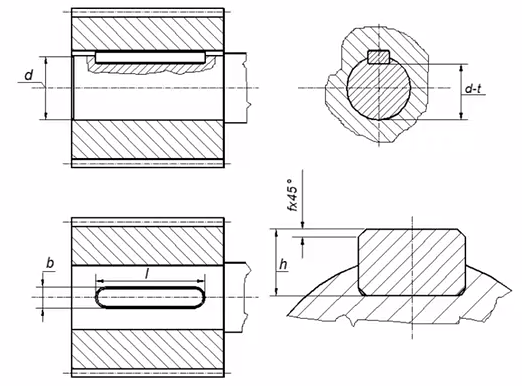
\includegraphics[width=\linewidth]{retesz}
	\caption{Reteszkötés méretei}
\end{wrapfigure}
\parbox{.5\textwidth}{
\begin{outline}
	\1 adatok
		\2 $d=60$ mm
		\2 $l=140$ mm
		\2 $b=18$ mm
		\2 $h=11$ mm
		\2 $t=6$ mm
		\2 $f=0.6$ mm
		\2 átvitt nyomaték: $T=1400$ Nm
		\2 Mekkorák a kötés igénybevételei?
\end{outline}}
\begin{outline}
	\1 megoldás
		\2 felületi nyomás
			\3 $F = \frac{2T}{d} = 46667$ N
			\3 $A_\text{p} = (h-t-f)(l-h) = 537\text{ mm}^2$
			\3 $p=\frac{F}{A_\text{p}}=86.9$ MPa
		\2 nyírás
			\3 $A_\tau = bl=2520\text{ mm}^2$
			\3 $\tau=\frac{F}{A_\tau}=18.5$ MPa
		\2 különlegességek elemzése
			\3 a tengelyben ébredő feszültség: $\tau=\frac{T}{I_\text{p}}\frac{d}{2}=33$ MPa
			\3 $I_\text{p}=\frac{d^4\pi}{32}=1272.345\text{ mm}^2$ (bevágás elhanyagolva)
\end{outline}
